

\chapter{Global Average Temperature}

%%%%%%%%%%%%%%%%%%%%%%%%%%%%%%%%%%%%%%%%%%%%%
\section*{Equipment List}

\begin{multicols}{2}   % change 2 -> 3 for three columns
\begin{equipment}
  \item Ruler
  \item Meter Stick
  \item IR Thermometer ``gun''
  \item Masking Tape
  \item incandescent lamp
  \item Computer
\end{equipment}
\end{multicols}

\vspace{0.5cm}
\noindent {\bf Note:} When you arrive at your table, clear a space on your table that is approximately half the area and mark it off with masking tape.  Then \underline{turn on the lamp} so that it it pointing down at one portion of that empty space.  You are ``pre-heating'' the table for measurements we will make below.

%%%%%%%%%%%%%%%%%%%%%%%%%%%%%%%%%%%%%%%%%%%%%
\section{Introduction and Definitions}

Today we consider the {\em Global Average Temperature}, which we have seen is the primary measure used to specify tha degree of global climate change over time.  Specifically, we will perform some experiments and analyses to mimic the process by which this quantity is calculated.  Obviously, there are many details that are used by professional climatologists that will will ignore, but we will focus on the two most important ideas: {\em area-weighted average} and {\em temperature anomalies}.

 The {\bf global average temperature} at a given moment in time, is defined to be (and calculated as) the weighted average of the temperature at every point on Earth, with weight for a given point being the area fraction assigned to that point.  For example, if we restricted ourselves to just the United States, we could {\em estimate} the ``US average temperature'' as:
 	%
	\begin{equation*}
	T_\text{US,avg} = T_\text{MI} \frac{A_\text{MI}}{A_\text{USA}} + T_\text{IN} \frac{A_\text{IN}}{A_\text{USA}} + T_\text{IL} \frac{A_\text{IL}}{A_\text{USA}} + \cdots
	\end{equation*}
	%
where you can see that the temperature value assigned to a state is weighted by the fraction of area (measured, e.g., in square kilometers) that state has in the total area of the US.  This can be written equivalently as
 	%
	\begin{equation*}
	T_\text{US,avg} = \frac{T_\text{MI} \, A_\text{MI} +  T_\text{IN} \,  A_\text{IN} +  T_\text{IL} \,  A_\text{IL} + \cdots}{A_\text{USA} }
	\end{equation*}
	%
This is a {\em weighted average} because the sum of all the factors in the numerator, $A_\text{MI} + A_\text{IN} + A_\text{IL} + \ldots$, adds up exactly to the value in the denominator (or, in the first question, the sum of all the weights, e.g., $\frac{A_\text{MI}}{A_\text{USA}}$, add up to one).  The calculation above would only be an estimate of the average temperature, because we have used only 50 points (one for each state) instead of ``all'' points in the US.  To improve our estimate\footnote{Technically: when the global average temperature is calcuated, the discrete temperature measurements at weather stations are used to produce a continuous ``function'' of temperature at every point on earth by interpolation between the stations; then that continuous function is ``integrated'' (calculus) over the total area.}, we could use multiple points per state (perhaps using a thermometer in each major city). Today we will perform a number of calculations to demonstrate this technique.

However, it is not actually the average temperature that is used to track climate change, but what is called the {\bf global average temperature anomaly}.  The average temperature anomaly is calculated as follows.  (1) A {\em reference time range} is chosen (usually a span of a decade or more, e.g., 1950--1980), over which temperatures will be averaged to determine a (local) reference temperature value. (2) At each thermometer location, the {\em local reference temperature} is calculated as an average over the reference time range. (3) The temperature anomaly (over time) at a given thermometer is calculated by subtracting off the local reference temperature from all temperature values.  (4) An area-weighted average of the temperature anomalies is calculated over the entire Earth. 


\section{Experiments and Activities}


\subsection{Temperature Anomalies}

Recall Figure 2.1 from the Dessler textbook, showing the temperature over time for two Texas cities, and then their respective temperature anomalies:
%
\begin{center}
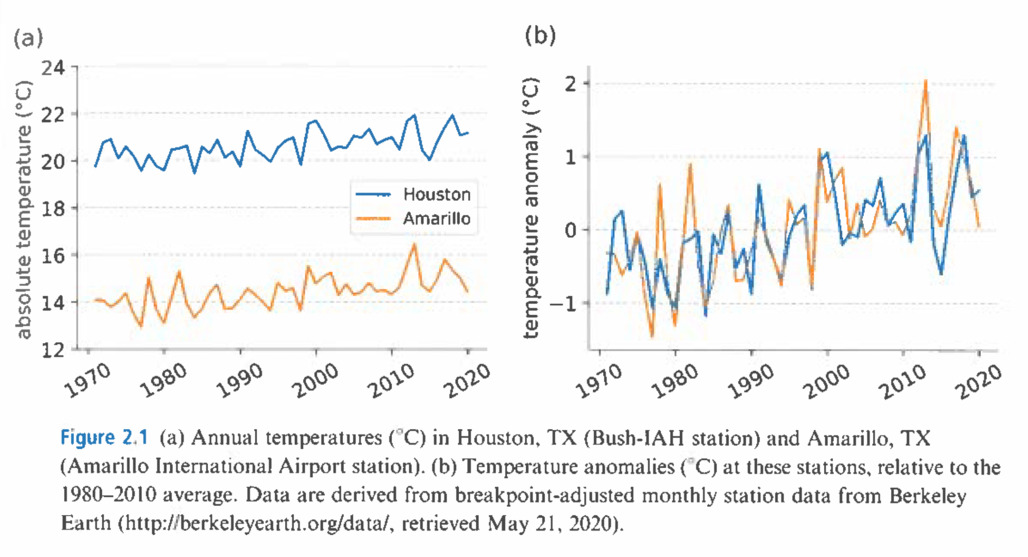
\includegraphics[width=\textwidth]{images/02_dessler_amarillo-vs-houston_fig2-1.jpg}
\end{center}
%
Use the similar graph below, for two Michigan cities.  (i) Determine a reference time period (ii) Estimate the refernece temperature for each (iii) Make an anomaly temperature timescale at right, and plot the values at three years for each city.
%
\begin{center}
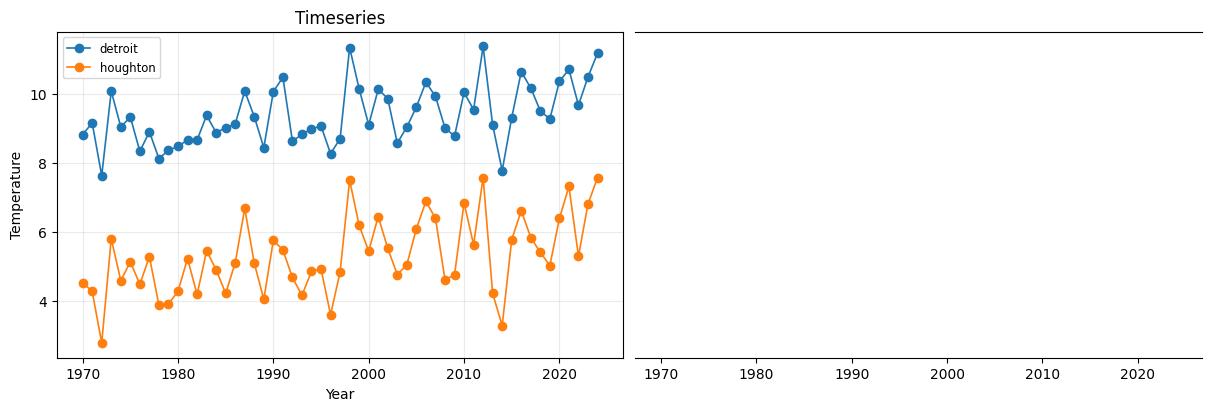
\includegraphics[width=0.9\textwidth]{images/02_detroit-houghton_temperatures.png}
\end{center}
%


\subsection{The approach to an average}

Find the dataset of your own collected temperature measurements (submitted by you and your classmates to the google form this past week) in the ``Results'' link on Blackboard.  For each of the two types of temperatures (air and sky) perform the following analysis:
	%
	\begin{itemize}
	\item Copy the data from the spreadsheet of all data into your own Google sheet (or Excel spreadsheet).  
	\item Clean the data column to make sure it contains only one numerical value per row. Save the single column of cleaned data as a csv file.
	\item Find the ``Scatter-Histogram-Average'' code on Blackboard.  Copy the blocks of code into a new Google Colab notebook. (This step does not need to be done twice).
	\item Run the code blocks. The last block will prompt you to upload your csv file and then make a plot.
	\end{itemize}


\subsection{Global average temperature (of your table)}

Perform a sequence of area-weighted averages of the temperature of your table in the previously marked off region, by completing the following steps:
	%
	\begin{enumerate}
	\item Measure the total area that you have marked off and record this value.
	\item Choose one point in the total area and measure the temperature using your IR thermometer gun.  This is {\bf Estimate 1}.
	\item Using masking tape, partition your total area into 3--4 smaller areas.  Measure the area of each one and record their values.  Also draw a picture to show the way you have partitioned and to give names to the sub-areas (e.g., $A_1$, $A_2$, etc).  
	\item Measure and record the temperature at one point in each of the sub-areas. Create a table with columns [name, area (units),  Temperature (units)].
	\item Using the method described above (average US temperature), calculate an area-weighted temperature from your data. This is {\bf Estimate 2}.
	\item Subdivide your table even further, such that you have about twice as many sub-areas.  Repeat steps 3--5 to calculate {\bf Estimate 3}.
	\end{enumerate}


\subsection{Global average temperature (of the Earth land surface)}

We will now attempt to find the global average temperature anomaly for the Earth.   Find the ``Get annual temperature data for one location'' code on Blackboard, and import the code blocks into a new Google Colab notebook.  We will make three estimates:
	%
	\begin{itemize}
	\item {\bf Estimate 1:} Using only one location on Earth (your choice).
	\item {\bf Estimate 2:} Using one location on each continent (again, your choice per continent).
	\item {\bf Estimate 3:} Using about twice as many locations, spread out across the Earth.
	\end{itemize}
	%
In each trial you will take the following steps:
	%
	\begin{enumerate}
	\item Use the ``Get annual temperature data'' code to download an annual average temperature dataset for one or more location over the 1970--2024 time range.
	\item Choose a time range over which to determine the local reference average (e.g., 1970--1990).
	\item Open this csv file (in Google sheets or Excel), and highlight the cells in that reference time range to find the reference average value.
	\item Use the spreadsheet tools to make a new temperature anomaly column, in which the reference average is subtracted off from the temperature.
	\item In Estimates 2 and 3, where you have multiple locations, create a new spreadsheet with a single date column at left and then a temperature anomaly column for each location.
	\end{enumerate}
	%
To make the global average calculation, we will need to edit this file in a few additional steps:
	%
	\begin{itemize}
	\item Look up online the surface area of each continent in square kilometers and record them.  To make these values more understandable, let's convert each into units of ``Michigan mitten''. The lower peninsula of Michigan has an area of almost exactly 100,000 square kilometers.  So you can divide each continental area by that value to obtain the area in ``mittens''.  
	\item In your multiple location spreadsheet, add two blank rows at top.  For each anomaly column, put the name in the first row, and the area (in mittens) in the second row.  In the first column (of dates) you can leave the first two rows blank.
	\item Locate the ``Get weighted average of timeseries'' code on blackboard and import the blocks into Colab.  It will allow you to import your csv file. If you use the format prescribed above (two extra rows above the temperature vs time data) then it should produced a weighted temperature anomaly graph.
	\end{itemize}





 